% =====================================================================
%  Certifying Optimal Experimental Design for Battery Aging
%  Statistics Honors Thesis Proposal (STAT 29900) -- mini-thesis format
%  Nathan Chenwei Hu, for Prof. Mihai Anitescu
%  Compile: pdflatex twice (TOC, cross-refs, back-references)
%  v3 (Oct 2026): data section corrected against the released data;
%  new Section 7 "Preliminary Results" (figures in figs/).
% =====================================================================
\documentclass[11pt,letterpaper]{article}
\usepackage[T1]{fontenc}
\usepackage[utf8]{inputenc}
\IfFileExists{lmodern.sty}{\usepackage{lmodern}\newcommand{\MicrotypeOpts}{}}{\newcommand{\MicrotypeOpts}{expansion=false}}
\usepackage[margin=1in,top=0.9in,bottom=0.9in]{geometry}
\expandafter\usepackage\expandafter[\MicrotypeOpts]{microtype}
\usepackage{amsmath,amssymb}
\usepackage{booktabs,tabularx,longtable,array,ragged2e}
\usepackage{graphicx}
\usepackage{float}
\usepackage{enumitem}
\usepackage{titlesec}
\usepackage[dvipsnames]{xcolor}
\usepackage[colorlinks=true,linkcolor=BrickRed,citecolor=RoyalBlue,urlcolor=RoyalBlue,linktoc=all,backref=page,
  pdftitle={Certifying Optimal Experimental Design for Battery Aging},pdfauthor={Nathan Chenwei Hu}]{hyperref}
\usepackage{hyphenat}
\usepackage{cleveref}
\renewcommand*{\backref}[1]{}
\renewcommand*{\backrefalt}[4]{\ifcase #1 (not cited)\or (cited on p.~#2)\else (cited on pp.~#2)\fi}

\titleformat{\section}{\normalfont\large\bfseries}{\thesection.}{0.6em}{}
\titleformat{\subsection}{\normalfont\normalsize\bfseries}{\thesubsection}{0.6em}{}
\titleformat{\subsubsection}{\normalfont\normalsize\itshape\bfseries}{\thesubsubsection}{0.6em}{}
\titlespacing*{\section}{0pt}{1.6ex plus 0.4ex}{0.8ex}
\titlespacing*{\subsection}{0pt}{1.1ex plus 0.3ex}{0.5ex}
\titlespacing*{\subsubsection}{0pt}{0.9ex plus 0.3ex}{0.4ex}
\setlist[itemize]{leftmargin=1.4em,itemsep=0.2ex,topsep=0.4ex,parsep=0pt}
\setlist[enumerate]{leftmargin=1.6em,itemsep=0.2ex,topsep=0.4ex,parsep=0pt}
\setlength{\parskip}{0.5ex plus 0.2ex}
\setlength{\parindent}{0pt}
\newcolumntype{L}{>{\RaggedRight\arraybackslash}X}
\renewcommand{\arraystretch}{1.12}
\newcommand{\dash}{\,---\,}
\newcommand{\ph}[1]{\textcolor{red}{\textbf{[PLACEHOLDER: #1]}}}
\newcommand{\RQ}[1]{\textbf{RQ#1}}
\graphicspath{{figs/}}

\begin{document}

\begin{center}
  {\LARGE\bfseries Certifying Optimal Experimental Design\\[0.2em] for Battery Aging Characterization}\\[0.6em]
  {\large Admissibility Diagnostics, Validity of Uncertainty, and Robust Designs}\\[0.8em]
  {\itshape Statistics Honors Thesis Proposal (STAT 29900)}\\[0.4em]
  {\small Nathan Chenwei Hu}\\[0.4em]
  {\small Advisor: Prof. Mihai Anitescu}\\[0.4em]
  {\small Second Reader: Prof. Chibueze Amanchukwu}\\[0.4em]
\end{center}

\begin{abstract}
\noindent Model-based optimal experimental design (OED) promises to make battery aging campaigns, among the slowest and most expensive experiments in battery research, more informative per cell. The first prospective test on real cells, a 279-cell two-stage study by Stroebl et al., gave a split result: OED reduced the uncertainty of a targeted calendar-aging parameter by 28\% but increased the uncertainty of targeted cycle-aging parameters by more than an order of magnitude. This thesis asks whether such outcomes can be predicted in advance and prevented by design. Using public aging datasets, it (i) constructs admissibility diagnostics from pilot data (identifiability, model adequacy, and noise structure) and tests whether they anticipate the observed success and failure; (ii) measures the coverage of bootstrap, Fisher-information, and profile-likelihood intervals at realistic campaign sizes; and (iii) evaluates compromise, Bayesian, and maximin designs that hedge against model error. The intended outcome is a practitioner checklist for when OED can be trusted.
\end{abstract}

\vspace{0.3em}\hrule\vspace{0.4em}
{\small \textbf{Document overview:} Sections 1--9 are a draft of the thesis itself; red markers \ph{\ldots} indicate tasks to be done. \Cref{sec:prelim} reports the first analyses of the Stroebl data. Appendices A--C are addressed to Dr. Anitescu: logistics and timeline, my background and goals, and fallback plans for the thesis.}
\vspace{0.3em}\hrule
{\small\tableofcontents}
\vspace{0.4em}\hrule\vspace{0.8em}

% =====================================================================
\section{Introduction}

\subsection{Motivation}
Every lithium-ion battery loses capacity as it is used, and how quickly depends on how it is used. Predicting that loss requires an \emph{aging model} whose parameters are estimated from \emph{aging campaigns}: batches of cells cycled for months under different controlled stress conditions while their capacity is measured. These campaigns are the slowest and most expensive instrument in battery research, and all the products downstream, e.g., lifetime prediction, warranty models, battery-management logic, and the degradation-aware dispatch of grid storage \cite{xu2018,shi2017}, inherit both the parameter values and their uncertainty. However, the campaigns themselves are usually designed by full-factorial grids or one-factor-at-a-time intuition \cite{stroebl2026}, methods that do not exploit what is already known about the system.

\subsection{State of the art literature}
Model-based \emph{optimal experimental design} (OED) proposes to fix this: choose the stress conditions and the number of cells at each so that the resulting data are maximally informative about the model parameters, in the sense of the Fisher information. The idea has been tried on batteries at increasing levels of realism\dash for electrochemical parameters within a single cell \cite{park2018,pozzi2019,ozkan2025,mikesell2025}, for calendar-aging parameters with physics-based models \cite{movahedi2023}, and for aging campaigns with polynomial models \cite{forman2012,mathieu2017,benmarzouk2016}. The decisive test came in 2024--2026, when Stroebl et al.\ ran a prospective, 279-cell, two-stage campaign explicitly built to compare OED against conventional designs \cite{stroebl2024}. The result was split: for \textbf{\textit{calendar aging}} (the degradation characteristics triggered during \textit{storage} of battery cells without external current flow), OED cut the uncertainty of the temperature parameter by 28\%. However, for \textbf{\textit{cycle aging}} (the degradation caused by repeated \textit{charge and discharge cycling} of battery cells), it \emph{increased} the uncertainty of the targeted parameters by more than an order of magnitude \cite{stroebl2026}. The authors attribute the failure to model inadequacy and insensitive parameters, and list as open problems the development of admissibility criteria, robust identification methods, and ``checklist-style thresholds'' for when OED may be applied \cite{stroebl2026}.

\subsection{Research questions}
This thesis takes the above diverging result as the starting point. The question is no longer \emph{whether} OED can help battery aging studies as it demonstrably can succeed (in the case of calendar aging) and demonstrably can fail (in the case of cycle aging). My question is whether the success of OED can be \emph{predicted in advance} and its failure can be \emph{prevented by design}:
\begin{itemize}
  \item \RQ{1} (\textbf{Admissibility}): Can the conditions under which OED improves parameter estimation be turned into quantitative diagnostics computable from pilot data alone, and do those diagnostics correctly predict the observed success (calendar) and failure (cycle) in the public Stroebl campaign?
  \item \RQ{2} (\textbf{Validity}): Are the uncertainty statements produced under OED\dash bootstrap standard deviations, Cram\'er--Rao bounds, confidence intervals\dash actually valid, i.e.\ do they attain nominal coverage under the sample sizes, noise structures, and cell-to-cell heterogeneity of real campaigns?
  \item \RQ{3} (\textbf{Robustness}): Can designs be constructed that hedge against model error\dash compromise and maximin designs imported from the accelerated-degradation-testing literature\dash and would they have averted the observed failure at acceptable efficiency cost?
\end{itemize}

\subsection{Contributions and organization}
The intended contributions are (i) a pre-hoc admissibility diagnostic for OED in aging models, validated retrospectively on public data; (ii) the first coverage study of uncertainty quantification under optimal versus heuristic designs for battery aging; (iii) robust/compromise design formulations for aging campaigns with a retrospective counterfactual evaluation; and (iv) a practitioner checklist. \Cref{sec:background} gives the necessary background for battery aging and OED; \cref{sec:lit} reviews the literature paper by paper; \cref{sec:problem} states the problem; \cref{sec:data} describes the data and how each corpus is used; \cref{sec:method} gives the methodology and planned analyses; \cref{sec:prelim} reports preliminary results on the Stroebl data; \cref{sec:expected} states expected results and limitations.

% =====================================================================
\section{Background}\label{sec:background}

\subsection{Battery aging}
\begin{itemize}
  \item \textbf{What ages.} Capacity (charge the cell can hold; reported as state of health, SoH, relative to nameplate) and power (rising internal resistance). Cells are conventionally ``end of life'' at SoH $=80\%$.
  \item \textbf{Why it ages.} Growth of the solid-electrolyte interphase (SEI) consumes cyclable lithium; particle cracking removes active material; lithium plating occurs under fast or cold charging \cite{vetter2005}. The mechanisms are chemically distinct but all appear as a falling capacity curve.
  \item \textbf{Two types of aging.} \emph{Calendar aging} proceeds with time even at rest, driven by temperature and the state of charge (SoC) at which the cell sits. \emph{Cycle aging} is driven by use, through the C-rate (current normalized by capacity; 1C empties the cell in one hour), the depth of discharge (DoD), temperature, and the SoC window.
  \item \textbf{Cell-to-cell variation.} Nominally identical cells age at different rates; Stroebl et al.\ therefore test several cells at every condition\dash three per cycle-aging test point and six per calendar-aging test point \cite{stroebl2024} (\cref{sec:data-stroebl}).
  \item \textbf{Cost.} A cycler channel holds one cell for the duration of a test; the natural unit of experimental cost is the \emph{cell-month}.
\end{itemize}

\subsection{Semi-empirical aging models}\label{sec:models}
Mechanistic electrochemical models are too expensive to embed in design or dispatch, so the working standard is a \emph{semi-empirical} form: a smooth, monotone function of the stress factors with a handful of parameters. The forms used by Stroebl et al.\ are representative \cite{stroebl2026}. For calendar aging, relative capacity is
\begin{equation}\label{eq:cal}
Q^{\mathrm{cal}}_{\mathrm{rel}}(T,\mathrm{SoC},t;\theta^{\mathrm{cal}}) = 1-\mathrm{EOL}_C\, e^{-\theta_0^{\mathrm{cal}}\left(\frac1T-\frac1{T_{\mathrm{ref}}}\right)}\left(\tfrac{\mathrm{SoC}}{\mathrm{SoC}_{\mathrm{ref}}}\right)^{\theta_1^{\mathrm{cal}}}\left(\tfrac{t}{t_{\mathrm{ref}}}\right)^{\theta_2^{\mathrm{cal}}},
\end{equation}
where $\theta_0$ is an Arrhenius (activation-energy-like) temperature parameter, $\theta_1$ the SoC sensitivity, and $\theta_2$ the time exponent ($\theta_2=0.5$ is the classical square-root law). The cycle-aging model has the same structure with five factors\dash temperature, maximum SoC, charge and discharge C-rates, and DoD\dash and a throughput exponent, giving six parameters $\theta^{\mathrm{cyc}}_0,\ldots,\theta^{\mathrm{cyc}}_5$ \cite{stroebl2026}. The widely used graphite/LFP model of Wang et al.\ has the same power-law-in-throughput backbone with an Arrhenius factor \cite{wang2011}. The point for statistics: $\theta$ is not a table of constants but a vector estimated from noisy data, and its estimate inherits the quality of the design that produced the data. Note also that the factors enter \emph{multiplicatively and separably}: the model has no interaction terms, so the effect of, e.g., charge rate is assumed to be the same at every temperature and SoC (\cref{sec:prelim-cycle}).

\subsection{How aging data are produced}
Cells are assigned to different stress conditions, cycled (or stored) in temperature chambers, and periodically taken through a \emph{reference performance test} (RPT) that measures capacity. In the Stroebl campaign, RPTs came in three scopes to limit their own influence on aging, calendar-aging cells were disconnected from testers between RPTs to imitate storage, and 279 Samsung INR21700-50E cells (4.9\,Ah) were tested at 71 test points across two stages \cite{stroebl2024}. A campaign is therefore a design $\xi=\{(x_i,n_i)\}$: stress conditions $x_i$ and cell counts $n_i$, under a budget of channels and months.

\subsection{Optimal experimental design (OED)}\label{sec:oed}
Suppose measurements satisfy $y=f(x;\theta)+\varepsilon$ with independent noise of variance $\sigma^2$. The \emph{Fisher information matrix} (FIM) of a design $\xi=(x_1,\ldots,x_k)$ is
\begin{equation}\label{eq:fim}
\mathcal I(\theta;\xi)=\frac1{\sigma^2}\sum_{l=1}^{k}\nabla_\theta f(x_l;\theta)\,\nabla_\theta f(x_l;\theta)^{\!\top},
\end{equation}
and the Cram\'er--Rao bound says no unbiased estimator can have covariance below $\mathcal I^{-1}$ \cite{palm2022,stroebl2026}. OED chooses $\xi$ to make some scalar summary of $\mathcal I^{-1}$ small: the determinant (\emph{D-optimality}, the volume of the confidence ellipsoid), the trace (\emph{A-optimality}), or one diagonal element (the variance of one parameter\dash Palm et al.'s \emph{parameter-individual} pi-OED \cite{palm2022}).

Two complications drive this thesis.
\begin{enumerate}
    \item First, for nonlinear $f$ the FIM depends on the unknown $\theta$, so a design is only ``optimal'' at a guessed value; the Bayesian remedy averages the criterion over a prior for $\theta$, which Chaloner and Verdinelli derive from a unified decision-theoretic view of design \cite{chaloner1995}, and the practical remedy is \emph{multi-stage} design in which a pilot stage supplies the guess \cite{palm2022,stroebl2026}.
    \item Second, everything above assumes the model $f$ is correct and the noise is well-behaved; when either fails, the ``optimal'' design can be worse than a naive one (\cref{sec:sloppy}).
\end{enumerate}

\subsection{Accelerated degradation test planning in reliability statistics}\label{sec:adt}
Statisticians have studied ``choose stress levels and allocate units to learn a degradation model efficiently'' for decades under the name \emph{accelerated degradation testing} (ADT). Differences from the battery literature are instructive: degradation is modeled as a stochastic process (Wiener or gamma) rather than a deterministic curve plus noise; the objective is typically the asymptotic variance of a lifetime \emph{quantile at the use condition} rather than a parameter variance; optimal plans tend to use only one or two stress levels; and \emph{compromise plans} deliberately add a third level purely to check the assumed stress--parameter relationship \cite{limyum2011,amini2018,shen2018}. These are precisely the ingredients missing from battery OED.

\subsection{Sloppiness and model discrepancy}\label{sec:sloppy}
Many mechanistic models are \emph{sloppy}: the FIM has eigenvalues spanning many orders of magnitude, so most parameter combinations are practically unidentifiable. White et al.\ show that in this regime OED can backfire: it selects \emph{complementary} experiments that shrink the uncertainty ellipse, but in doing so makes mechanisms the model omits become relevant, so the best fit lands outside the model's valid region and predictive power drops even though parameters become identifiable \cite{white2016}. They quantify this with a simple ``hyper-model'' of model error. This is, as \cref{sec:lit-aging} argues and \cref{sec:prelim-cycle} begins to show in the data, what appears to have happened in the Stroebl cycle-aging arm.

% =====================================================================
\section{Literature Review}\label{sec:lit}

\subsection{OED for single-cell electrochemical parameter identification}
Most battery OED work designs the \emph{current profile} applied to \textbf{one cell} over hours so that electrochemical parameters become identifiable.
\begin{itemize}
    \item Park et al.\ derive sensitivity equations for an electrochemical model, group parameters by orthogonalized sensitivity, build a library of input profiles, and select the most informative by convex programming, validating on \textbf{one} 18650 NCA cell with lower voltage RMSE than standard cycles \cite{park2018}.
    \item Pozzi et al.\ performed Fisher-based nonlinear optimization for the single-particle model with electrolyte dynamics, first with the model as the plant and then with a P2D model standing in for the real cell, which serves as an early check of design under model mismatch \cite{pozzi2019}.
    \item Two 2025 papers from Ohio State replace the optimizer with reinforcement learning:
    \begin{itemize}
        \item Ozkan et al.\ use TD3 to shape excitation and report higher Fisher information and lower estimation error than nonlinear MPC and conventional tests \cite{ozkan2025}.
        \item Mikesell et al.\ run it in real time on hardware-in-the-loop \cite{mikesell2025}.
    \end{itemize}
    \item Movahedi et al.\ move to aging: with a closed-form SEI model they show that, in the kinetically limited regime, calendar tests at high SoC estimate SEI parameters most accurately, and use OED to pick storage SoCs \cite{movahedi2023}.
\end{itemize}
These studies all focus on studying the aging of \textbf{one} cell, and none of these addresses the allocation of \emph{many cells across various stress conditions over months}, which is the campaign/batch problem.

\subsection{Design of experiments for aging campaigns/batches}\label{sec:lit-aging}
\textbf{Linear-model D-optimality.} Forman et al.\ introduced OED to battery health experiments: a linear-in-parameters capacity model $H=U\beta$ lets classical D-optimality select CCCV cycles; 14 LiFePO$_4$ cells (10 for fitting, 4 for validation) were cycled for 429 days, and the authors note the absence of replicate trials as a limitation \cite{forman2012}. Mathieu et al.\ used a D-optimal design within the MOBICUS project for a graphite/LMO--NMC cell: 27 conditions over temperature (0--60$^\circ$C), SoC (0--100\%), and current (0, C/3, 1C), a quadratic response model for the degradation rate with a temperature--current interaction, $R^2=0.96$, validation on six mixed calendar/cycling tests to 1.08\% absolute error at 200 days, and a proposed 10-run D-optimal follow-up \cite{mathieu2017}; the MOBICUS protocols paper confirms that part of the campaign was built by D-optimal design \cite{benmarzouk2016}. The Rom\'an-Ram\'irez and Marco review catalogs these and other DoE studies across battery aging, formulation, and manufacturing \cite{roman2022}.

\textbf{Nonlinear pi-OED in simulation.} Palm, Stroebl and Palm formalize pi-OED as minimizing $(\mathcal I^{-1})_{ii}$ for a chosen parameter, demonstrate it on the calendar model \eqref{eq:cal} in computer experiments, and benchmark it against D-optimal, random, and Latin-hypercube designs: pi-OED wins on the targeted parameter while D-optimality gives lower variance on the others. They use bootstrapping to obtain estimator distributions and note that this ``is only feasible for computer experiments,'' relying on the Cram\'er--Rao bound in practice; code is public \cite{palm2022}.

\textbf{Prospective validation on real cells.} The Stroebl campaign \cite{stroebl2024} and its analysis \cite{stroebl2026} are the closest prior work and deserve a detailed account. Stage S1 used non-model-based designs: a full-factorial-type grid for calendar aging (11 of the 15 combinations of three temperatures and five SoCs, six cells each) and a conditioned Latin hypercube over five factors for cycle aging (25 test points, three cells each). Parameters were estimated by least squares and their uncertainty by blockwise bootstrapping ($n_{\mathrm{BS}}=10{,}000$) and by the FIM. The parameter with the largest relative Fisher standard deviation was then targeted in Stage S2 by pi-OED (S2b), while a parallel arm (S2a) continued the non-model-based design (\cref{tab:design} gives the cell counts per arm; in the calendar study the arms are not equal in size, and a third, manually chosen calendar arm was added). \emph{Calendar aging:} $\theta_0^{\mathrm{cal}}$ (relative SD 4.46\%, the largest) was targeted with four optimized test points\dash which, in the released metadata, all share a single storage condition (23\,$^\circ$C, 80\% SoC); its bootstrap SD fell from 89.01 (S1+S2a) to 63.78 (S1+S2b), a 28\% reduction. \emph{Cycle aging:} the current-rate parameters $\theta_2,\theta_3$ (relative SDs 23.8\% and 9.5\%) were targeted with twelve test points; their SDs \emph{rose} from 2.10 to 38.0 and from 32.5 to 399.6, and the estimate of $\theta_3$ drifted from $-12.8$ to $-284.6$\dash a parameter running along a practically unidentifiable direction. The authors' diagnosis: the model was inadequate ($R^2_{\mathrm{adj}}$ of 0.93, 0.87, 0.83 for the three cases against a validity threshold of 0.95; superlinear trajectories the model cannot represent), the targeted factors were not statistically significant (a leave-one-covariate-out comparison gave Mann--Whitney $p>0.05$), and the cycle-aging residuals failed a Shapiro--Wilk normality test. They also report two anomalies they could not fully explain: bootstrap distributions of $\theta_0^{\mathrm{cal}}$ from S1 and from S1+S2 that differ by more than $4\sigma$ although the second dataset contains the first, reproduced in a virtual experiment in which even the \emph{correct} model yields $4\sigma$-separated designs after 333 random draws; and systematic gaps between bootstrap and FIM variances, which they propose\dash tentatively\dash as a diagnostic of model validity or non-convergence \cite{stroebl2026}. Their stated open problems are robust identification methods, sensitivity analysis accounting for parameter interdependence, adaptive stage durations, and checklist-style admissibility thresholds.

\subsection{Accelerated degradation test planning}
Lim and Yum plan constant-stress ADTs under a Wiener-process degradation model, choosing stress levels and allocation proportions to minimize the asymptotic variance of the MLE of a lifetime quantile at the use condition; optimal plans involve one or two stress levels, so they add three-level compromise plans to check the stress--parameter relationship and give sensitivity procedures for uncertainty in the pre-estimated parameter \cite{limyum2011}. Amini et al.\ extend step-stress ADT with random stress-elevation times under a gamma process, optimizing threshold, sample size, measurement frequency, and termination time under a cost budget \cite{amini2018}. Shen et al.\ apply Wiener-process CSADT design to lithium-ion cells with discharge rate as the stress: 20 cells, C-rates from 1C to 10C, quadratic drift, a local-search optimizer over stress levels and allocation; the mean asymptotic variance of the median life falls from 37.9 to 19.2 and the optimal plan collapses from four stress groups to three \cite{shen2018}. This was a design calculation only; no validation on real data followed.

\subsection{Design under model error and observation noise}
White et al.\ (\cref{sec:sloppy}) provide the theory of OED failure under model discrepancy, with EGFR-signaling and DNA-repair models as examples, and argue for hierarchies of models rather than parameter estimation in a single model \cite{white2016}. Qi and Baker use local (FIM) and global (Sobol') sensitivity to optimize \emph{observation times} and show that correlated observation noise materially changes the optimal time points \cite{qibaker2025}\dash directly relevant to when RPTs should be scheduled, a design dimension no battery study has optimized.

\subsection{Why aging parameters matter downstream}
Shi et al.\ prove that rainflow-cycle-based degradation cost is convex, enabling its use in storage optimization with a subgradient method, demonstrated on the PJM regulation market \cite{shi2017}; Xu et al.\ build the marginal aging cost for market dispatch on a two-parameter stress function $\Phi(\delta)=5.24\times10^{-4}\delta^{2.03}$ taken from a single cited study, with no uncertainty attached \cite{xu2018}. Whatever uncertainty an aging campaign leaves in $\theta$ is inherited, unquantified, by these decisions.

\subsection{Synthesis: what is established and what is open}
\begin{tabularx}{\textwidth}{@{}p{4.6cm} L L@{}}
\toprule
\textbf{Question} & \textbf{Established} & \textbf{Open (this thesis)} \\
\midrule
Does OED help for aging models? & Yes for calendar aging (28\%), no for cycle aging, on real cells \cite{stroebl2026}; yes in simulation \cite{palm2022}; D-optimal linear designs \cite{forman2012,mathieu2017} & Predicting \emph{which} case one is in before spending cells (\RQ1) \\
Which criterion? & pi-OED vs.\ D/random/LH compared in simulation \cite{palm2022} & Not a headline question; treated as background \\
Are the uncertainties valid? & Bootstrap and CRLB reported; $4\sigma$ non-overlap and BS--FIM gaps observed but unexplained \cite{stroebl2026} & Coverage of intervals under design, noise, heterogeneity (\RQ2) \\
Robust designs? & Compromise/sensitivity plans exist for Wiener ADT \cite{limyum2011}; maximin ideas in biology \cite{white2016} & Never applied to battery aging; counterfactual on public data (\RQ3) \\
Heterogeneity? & Handled by replicate cells (3--6 per test point) \cite{stroebl2024} & Random-effects information and design \\
\bottomrule
\end{tabularx}

% =====================================================================
\section{Problem Statement}\label{sec:problem}

\subsection{Formal setting}
Let $Q(t;x,\theta)$ be a semi-empirical aging model (\cref{sec:models}) with stress condition $x$ and parameters $\theta\in\Theta\subset\mathbb R^p$. A campaign is a design $\xi=\{(x_i,n_i)\}_{i=1}^m$ subject to $\sum_i n_i\le N$ cells and a horizon of $M$ months, with RPTs at times $t_1<\dots<t_r$. Observed capacities are $y_{ijl}=Q(t_l;x_i,\theta)+b_{ij}+\varepsilon_{ijl}$, where $b_{ij}$ is a cell-level effect and $\varepsilon_{ijl}$ measurement noise; cells surviving the horizon are right-censored in lifetime. Estimation is by constrained least squares or maximum likelihood ($\theta$ physically admissible); uncertainty by bootstrap, by $\mathcal I^{-1}$, or by profile likelihood.

\subsection{The admissibility assumptions and their failure modes}
Stroebl et al.\ state three prerequisites for OED to deliver its promised gain \cite{stroebl2026}: \textbf{R1} the model reflects the true behavior without redundant parameters; \textbf{R2} repeated measurements are homoscedastic normal around the model; \textbf{R3} pilot estimates are close enough to the truth for the computed design to be near-optimal. In their data, R1 failed in the cycle arm (inadequate fit, insensitive factors), R2 failed in the cycle arm (non-normal residuals), and R3 was questioned in the calendar arm (the $4\sigma$ non-overlap). These assumptions are stated qualitatively in the existing literature and this thesis seeks to quantify them.

\subsection{Research questions}
\begin{itemize}
  \item \RQ{1} \textbf{Admissibility diagnostic.} Define statistics $D_1$ (identifiability: spectrum and condition of $\mathcal I(\hat\theta_{S1};\xi_{S1})$, sloppiness), $D_2$ (adequacy: lack-of-fit relative to replicate noise, plus a discrepancy hyper-model in the spirit of \cite{white2016} evaluated over the \emph{proposed} S2 stress range), and $D_3$ (noise: residual normality/heteroskedasticity), all computable from S1 data. Hypothesis: $(D_1,D_2,D_3)$ computed from Stroebl S1 predict the calendar success and cycle failure before S2 is seen.
  \item \RQ{2} \textbf{Coverage.} For intervals from blockwise bootstrap, FIM/CRLB, and profile likelihood, under designs (FF, cLH, pi-OED, D-optimal), sample sizes matching real campaigns, and noise and heterogeneity conditions (normal iid; heteroskedastic; non-normal as in the cycle arm; random effects), estimate actual coverage and interval width. Hypothesis: the $4\sigma$ non-overlap and BS--FIM gaps are small-sample coverage failures, not evidence of non-convergence.
  \item \RQ{3} \textbf{Robust design.} Formulate compromise designs (extra stress level for model checking \cite{limyum2011}) and maximin/Bayesian designs over a set of model forms and priors \cite{chaloner1995}; evaluate retrospectively on Stroebl and Severson corpora whether such a design would have avoided the cycle-aging failure and at what efficiency cost in the calendar case.
\end{itemize}

% =====================================================================
\section{Data}\label{sec:data}

\subsection{Stroebl multi-stage aging dataset (primary)}\label{sec:data-stroebl}
\textbf{What it is.} 279 Samsung INR21700-50E cells (4.9\,Ah) aged under 71 test points in two stages (141 cells in S1, 138 in S2); calendar (132 cells, 22 test points, six cells each) and cycle (147 cells, 49 test points, three cells each) sub-studies; S1 non-model-based (FF / cLH); S2 split into a non-model-based arm (S2a), a pi-OED arm (S2b), and, for calendar aging only, a third \emph{manually chosen} arm; periodic RPTs of three scopes; raw cycler time series as CSV with per-cell metadata, CC-BY-4.0 on figshare \cite{stroebl2024}. \Cref{tab:design} gives the design by arm.

\textbf{Calendar factors.} $T\in\{10,23,45\}^\circ$C and SoC $\in\{5,20,50,80,100\}\%$, but S1 covers only 11 of the 15 combinations: SoC 5, 50, and 100\% at all three temperatures, and SoC 20 and 80\% at 45\,$^\circ$C only. S2a fills three of the gaps (10\,$^\circ$C/20\%, 10\,$^\circ$C/80\%, 23\,$^\circ$C/20\%); the pi-OED arm places all four of its test points at the remaining gap, 23\,$^\circ$C/80\%; the manual arm tests the new levels SoC 65\% and 90\% at 23 and 45\,$^\circ$C. The FF and pi-OED arms of S2 stay at SoC $\le80\%$ after the non-monotonic behavior above 80\% in S1 \cite{stroebl2026}; the manual arm goes to 90\%.

\textbf{Cycle factors.} $T\in\{23,35,45\}^\circ$C (three levels), SoC$_{\max}\in[0.2,0.8]$, $C_{\mathrm{ch}}\in[0.05,1.0]$, $C_{\mathrm{dch}}\in[0.05,2.0]$, DoD $\in[0.2,0.6]$ \cite{stroebl2026}, with DoD constrained by SoC$_{\max}$ (high DoD only at high SoC$_{\max}$). \ph{Check the continuous factor ranges against the released metadata, which suggest DoD values below 0.2.} The twelve pi-OED test points use only four distinct conditions, all at the high-stress corner (\cref{sec:prelim-design}). Outliers were flagged by the authors (2.56\% of calendar points) \cite{stroebl2026}.

\begin{table}[H]
\centering\small
\caption{Design of the Stroebl campaign by sub-study, stage, and arm, as reconstructed from the released metadata (\texttt{experiments\_meta.csv}).}\label{tab:design}
\begin{tabular}{@{}llllrr@{}}
\toprule
Sub-study & Stage & Arm & Design & Cells & Test points \\
\midrule
Calendar & S1 & pilot & full factorial (11 of 15) & 66 & 11 \\
Calendar & S2 & S2a & full factorial (gap filling) & 18 & 3 \\
Calendar & S2 & S2b & pi-OED & 24 & 4 \\
Calendar & S2 & manual & hand-chosen & 24 & 4 \\
Cycle & S1 & pilot & conditioned Latin hypercube & 75 & 25 \\
Cycle & S2 & S2a & conditioned Latin hypercube & 36 & 12 \\
Cycle & S2 & S2b & pi-OED & 36 & 12 \\
\midrule
\multicolumn{4}{@{}l}{Total} & 279 & 71 \\
\bottomrule
\end{tabular}
\end{table}

\textbf{Pipeline (done).} The figshare record (version 1) holds 280 files: the metadata table and one zip per cell. All files were checked against figshare's MD5 checksums (279 match; one has a mismatched published checksum but the correct size and an intact archive). Each zip holds one cell's entry test (ET, at 10/23/45\,$^\circ$C), alternating cycling blocks and RPTs (check-up CU; extended check-up exCU), and an end test (AT). Capacity at each RPT is computed as $\int |I|\,dt$ over the 1C capacity discharge (step code 22, 4.15$\to$2.50\,V); throughput for cycle cells is $\int|I|\,dt$ summed over the cycling blocks before each RPT and reported as equivalent full cycles, EFC $=$ Ah$/(2\times4.9)$. The result is a tidy table of 2{,}766 RPT records for all 279 cells (cell, arm, stress factors, RPT index and kind, date, capacity, EFC); counts reconcile exactly with the paper (279 cells, 71 test points). Three data pitfalls had to be resolved: (i) each file name is reused for two different cells, one per stage; (ii) the authors' internal cell serial is not unique (261 distinct values for 279 cells), so cells are identified by file name plus stage, with stage inferred from the measurement start date (141 cells started in Sep--Oct 2021, 138 in Dec 2022--Feb 2023); (iii) a few per-test metadata files are missing or contain malformed dates, which affect only those tests.

\textbf{Why it is ideal.} It is the only public dataset with an OED arm and a matched control arm; the fitted models, estimates, bootstrap SDs, and FIM values are published (Tables D.2--D.3 of \cite{stroebl2026}), so the first task is exact reproduction; and the S1/S2 split makes a genuine \emph{prospective-style} validation of \RQ1 possible: compute diagnostics on S1 only, predict, then check against S2.

\textbf{What will be done with it.} (a) Reproduce the published S1 fits, bootstrap SDs, and FIM relative SDs for both sub-studies. (b) Compute $D_1$--$D_3$ on S1 and test the \RQ1 prediction. (c) Use the fitted models as simulation truths for \RQ2. (d) Re-run the design step with compromise/maximin criteria for \RQ3 and compare against the actual S2b. \ph{Confirm from \cite{stroebl2024,stroebl2026} which RPT scopes enter the published fits (the ET and AT capacities differ systematically from neighboring CUs), what distinguishes the four calendar pi-OED test points, and what the manual calendar arm was for.}

\subsection{Severson et al.\ (MATR) LFP fast-charging dataset}
124 commercial LFP/graphite cells cycled to failure under 72 fast-charging protocols, cycle lives from roughly 150 to 2{,}300 \cite{severson2019}. \textbf{Role:} a second chemistry and a second failure regime (fast charging) for \RQ2 simulation truths and for \RQ3 retrospective design: treating the full-corpus fit as ground truth $\theta^*$, candidate designs select $k$-cell subsets and their realized error and coverage are compared with what the criteria predicted. Limitation: single temperature, so the Arrhenius parameter is not identifiable here\dash itself a useful \RQ1 test case. \ph{Parse via BatteryML; extract capacity-vs-cycle per cell; confirm protocol metadata.}

\subsection{Sandia National Laboratories commercial-cell study}
LFP, NCA, and NMC cells cycled over a grid of discharge rate, DoD, and temperature for multiple years \cite{preger2020}, hosted on batteryarchive.org. \textbf{Role:} the temperature variation Severson lacks, so the activation-energy parameter is identifiable; cross-chemistry check of whether the \RQ1 diagnostic transfers. \ph{Download from batteryarchive.org; harmonize capacity units and RPT cadence across chemistries.}

\subsection{Data-to-question map}
\begin{tabularx}{\textwidth}{@{}p{3.4cm} L L L@{}}
\toprule
\textbf{Corpus} & \RQ{1} Admissibility & \RQ{2} Coverage & \RQ{3} Robust design \\
\midrule
Stroebl (calendar + cycle) & Primary validation: S1 $\to$ predict S2 outcome & Simulation truths from published fits; real-data replicate structure & Counterfactual redesign of S2b \\
Severson (LFP) & Non-identifiability test case (no temperature variation) & Subsampling coverage under heterogeneity & Retrospective $k$-cell design benchmark \\
Sandia (multi-chemistry) & Transfer of diagnostic across chemistries & Heteroskedastic/long-horizon noise & Compromise-plan evaluation with temperature \\
\bottomrule
\end{tabularx}

All data are public; nothing lab-owned is used.

% =====================================================================
\section{Methodology and Planned Analyses}\label{sec:method}

\subsection{Models, estimation, and uncertainty (shared infrastructure)}
\begin{itemize}
  \item \textbf{Models.} The Stroebl calendar and cycle forms \cite{stroebl2026} as published; the Wang power law \cite{wang2011} for LFP corpora; a mixed-effects extension with cell-level random effects on the severity term; optionally a Wiener-process alternative in the ADT tradition \cite{limyum2011} for comparison of information structure.
  \item \textbf{Estimation.} Constrained nonlinear least squares / MLE (Ipopt via JuMP, or SciPy), with parameter bounds for physical admissibility.
  \item \textbf{Uncertainty.} Blockwise bootstrap exactly as in \cite{stroebl2026} (blocks = cells), FIM/CRLB, profile likelihood; for mixed effects, the marginal-likelihood information.
  \item \ph{Reproduce Tables D.2--D.3 of Stroebl 2026 to within bootstrap Monte Carlo error; document any discrepancy.}
\end{itemize}

\subsection{\RQ1: Admissibility diagnostics}
\subsubsection{Construction}
\begin{itemize}
  \item $D_1$ \textbf{identifiability:} eigen-decomposition of $\mathcal I(\hat\theta_{S1};\xi_{S1})$; condition number, sloppiness spectrum, and the projection of each targeted parameter onto small-eigenvalue directions. Prediction rule: OED targeting a parameter that lies mostly in a sloppy direction cannot reduce its variance by adding data along the same directions.
  \item $D_2$ \textbf{adequacy:} pure-error lack-of-fit test using replicates; a discrepancy hyper-model (an additive flexible term in the stress factors, including pairwise interactions) fitted on S1 and \emph{extrapolated} to the proposed S2 stress region, measuring whether the model's validity region contains the proposed design, which is essentially the mechanism of \cite{white2016}. A simple companion statistic, motivated by \cref{sec:prelim-design}: how much S1 data supports the model at the proposed design points (e.g.\ the number of S1 test points within a neighborhood of each proposed point in the joint factor space).
  \item $D_3$ \textbf{noise:} residual normality and variance-vs-level regressions, since pi-OED's FIM assumes homoscedastic normal noise (R2); the replicate-spread analysis of \cref{sec:prelim-noise} is a model-free first version.
\end{itemize}
\subsubsection{Validation protocol}
Compute $(D_1,D_2,D_3)$ on Stroebl S1 for both sub-studies without using S2; state a prediction (gain expected / not expected) with a pre-registered threshold; then compare to the published S2 outcomes. Repeat on Severson and Sandia by treating a subset as ``S1.'' The exploratory analysis in \cref{sec:prelim} has already looked at S2 data; to keep the \RQ1 test honest, the diagnostics and their thresholds will be fixed using S1 data only, and the Severson and Sandia replications, which have not been examined, serve as the clean out-of-sample test. \ph{Pre-register thresholds for $D_1$--$D_3$ on S1 data only; record in the repository.} \ph{Figure: FIM eigen-spectra for calendar vs.\ cycle S1 models; table of diagnostics vs.\ realized S2 gain.}

\subsection{\RQ2: Coverage of uncertainty statements}
\subsubsection{Simulation design}
Truths: published Stroebl fits; Severson and Sandia fits. Factors: interval method (blockwise bootstrap, FIM/CRLB, profile likelihood, mixed-effects) $\times$ design (FF, cLH, pi-OED, D-optimal) $\times$ cells per condition (1--6) $\times$ noise (normal iid; heteroskedastic; heavy-tailed as observed in the cycle arm) $\times$ heterogeneity (none; random effects). Noise levels will be calibrated to the empirical replicate spread (\cref{sec:prelim-noise}). Outputs: empirical coverage at 95\%, mean width, and the distribution of the BS--FIM ratio.
\subsubsection{Specific hypotheses}
(i) The $4\sigma$ non-overlap in \cite{stroebl2026} is reproduced by small-sample bootstrap bias in nonlinear least squares with $\sim$5 design points and disappears with cells per condition or with profile-likelihood intervals. (ii) The BS--FIM ratio is a usable diagnostic of misspecification only above a sample-size threshold, which will be quantified. \ph{Implement simulation harness; run the factorial; produce coverage tables and the BS--FIM diagnostic figure.}

\subsection{\RQ3: Robust and compromise designs}
\subsubsection{Formulations}
\begin{itemize}
  \item \textbf{Compromise design:} pi-OED/D-optimal with a constraint reserving a fraction of cells for a validation stress level outside the optimized set, following \cite{limyum2011}.
  \item \textbf{Bayesian design:} expected criterion over a prior for $\theta$ built from S1 bootstrap draws \cite{chaloner1995}.
  \item \textbf{Maximin over model forms:} worst-case criterion over a small family (with/without current-rate factors, with/without superlinear term, with/without a charge-rate$\times$temperature interaction), so that a design must be informative under every plausible model\dash a direct response to the R1 failure.
  \item \textbf{Optimization:} exact designs as mixed-integer nonlinear programs; continuous relaxation over allocation weights, rounding, and exchange steps; implemented in JuMP with Ipopt.
\end{itemize}
\subsubsection{Counterfactual evaluation}
For the Stroebl cycle sub-study: compute each robust design from S1, then estimate the S2 outcome it would have produced by (a) simulation from the best available model and (b) nearest-neighbor reuse of actually tested S2 conditions. For the calendar sub-study: quantify the efficiency lost by hedging (the ``price of insurance''). For Severson: retrospective $k$-cell subset benchmark of realized error and coverage. \ph{Implement design optimizer; run counterfactuals; figure: efficiency-vs-robustness frontier.}

\subsection{Software and reproducibility}
Julia (JuMP, Ipopt, Distributions.jl) for design optimization; Python (pandas, SciPy, statsmodels; BatteryML for Severson) for data and estimation; Palm et al.'s public pi-OED code as the reference implementation \cite{palm2022}; one private GitHub repository with a pinned conda environment, a scripted and checksum-verified data download, seeds, and one notebook or script per figure.

% =====================================================================
\section{Preliminary Results}\label{sec:prelim}
This section reports the first, model-free look at the Stroebl data: the design as actually run, the capacity-fade curves, and the replicate noise. No model has been fitted yet; the observations below are hypotheses for the analyses of \cref{sec:method}, not conclusions. Unless noted, curves use the regular RPTs only (CU and exCU); the entry and end tests are excluded because their capacities differ systematically from the neighboring check-ups (e.g.\ for one calendar cell the end test reads 0.04\,Ah below the last CU taken 13 days earlier, about six times that cell's normal fade rate), which points to a protocol difference rather than aging. Capacity is reported relative to each cell's first regular RPT.

\subsection{Where the OED designs placed their cells}\label{sec:prelim-design}
\Cref{fig:design} shows the 49 cycle-aging test points in the five-dimensional factor space. The two non-model-based arms spread over the space as a Latin hypercube should, with the triangular SoC$_{\max}$--DoD region imposed by the physical constraint DoD $\le$ SoC$_{\max}$. The pi-OED arm does something entirely different: all twelve of its test points (36 cells) sit at one corner of the space, $T=45\,^\circ$C, SoC$_{\max}=0.8$, DoD $=0.6$\dash the maximum of each range\dash and vary only the two targeted factors, at four extreme combinations of charge and discharge rate: $(C_{\mathrm{ch}},C_{\mathrm{dch}})\in\{(1.00,2.00),(0.24,2.00),(1.00,0.26),(0.20,0.44)\}$. This is the classical shape of a locally optimal design (vary the targeted factors as far apart as possible; set the nuisance factors to maximum signal), and it mirrors the ADT finding that optimal plans concentrate on the fewest, most extreme levels \cite{limyum2011}.

The pilot stage supported that corner with a single test point (three cells), at moderate C-rates $(0.8, 0.6)$. Each pi-OED factor value lies within the range S1 covered, but the \emph{combination}\dash fast charging at 45\,$^\circ$C, high SoC, and high DoD\dash was never tested in S1. The design therefore relied on the model's separable, interaction-free structure (\cref{sec:models}) to transfer C-rate effects estimated elsewhere in the space to the region where physically the strongest interactions are expected (lithium plating and heating under fast charge). The calendar pi-OED arm is a useful contrast: its four test points share one interior condition, 23\,$^\circ$C/80\% SoC, bracketed by S1 data at the same temperature (SoC 50 and 100\%) and at the same SoC (45\,$^\circ$C)\dash and that arm succeeded.

\begin{figure}[H]
\centering
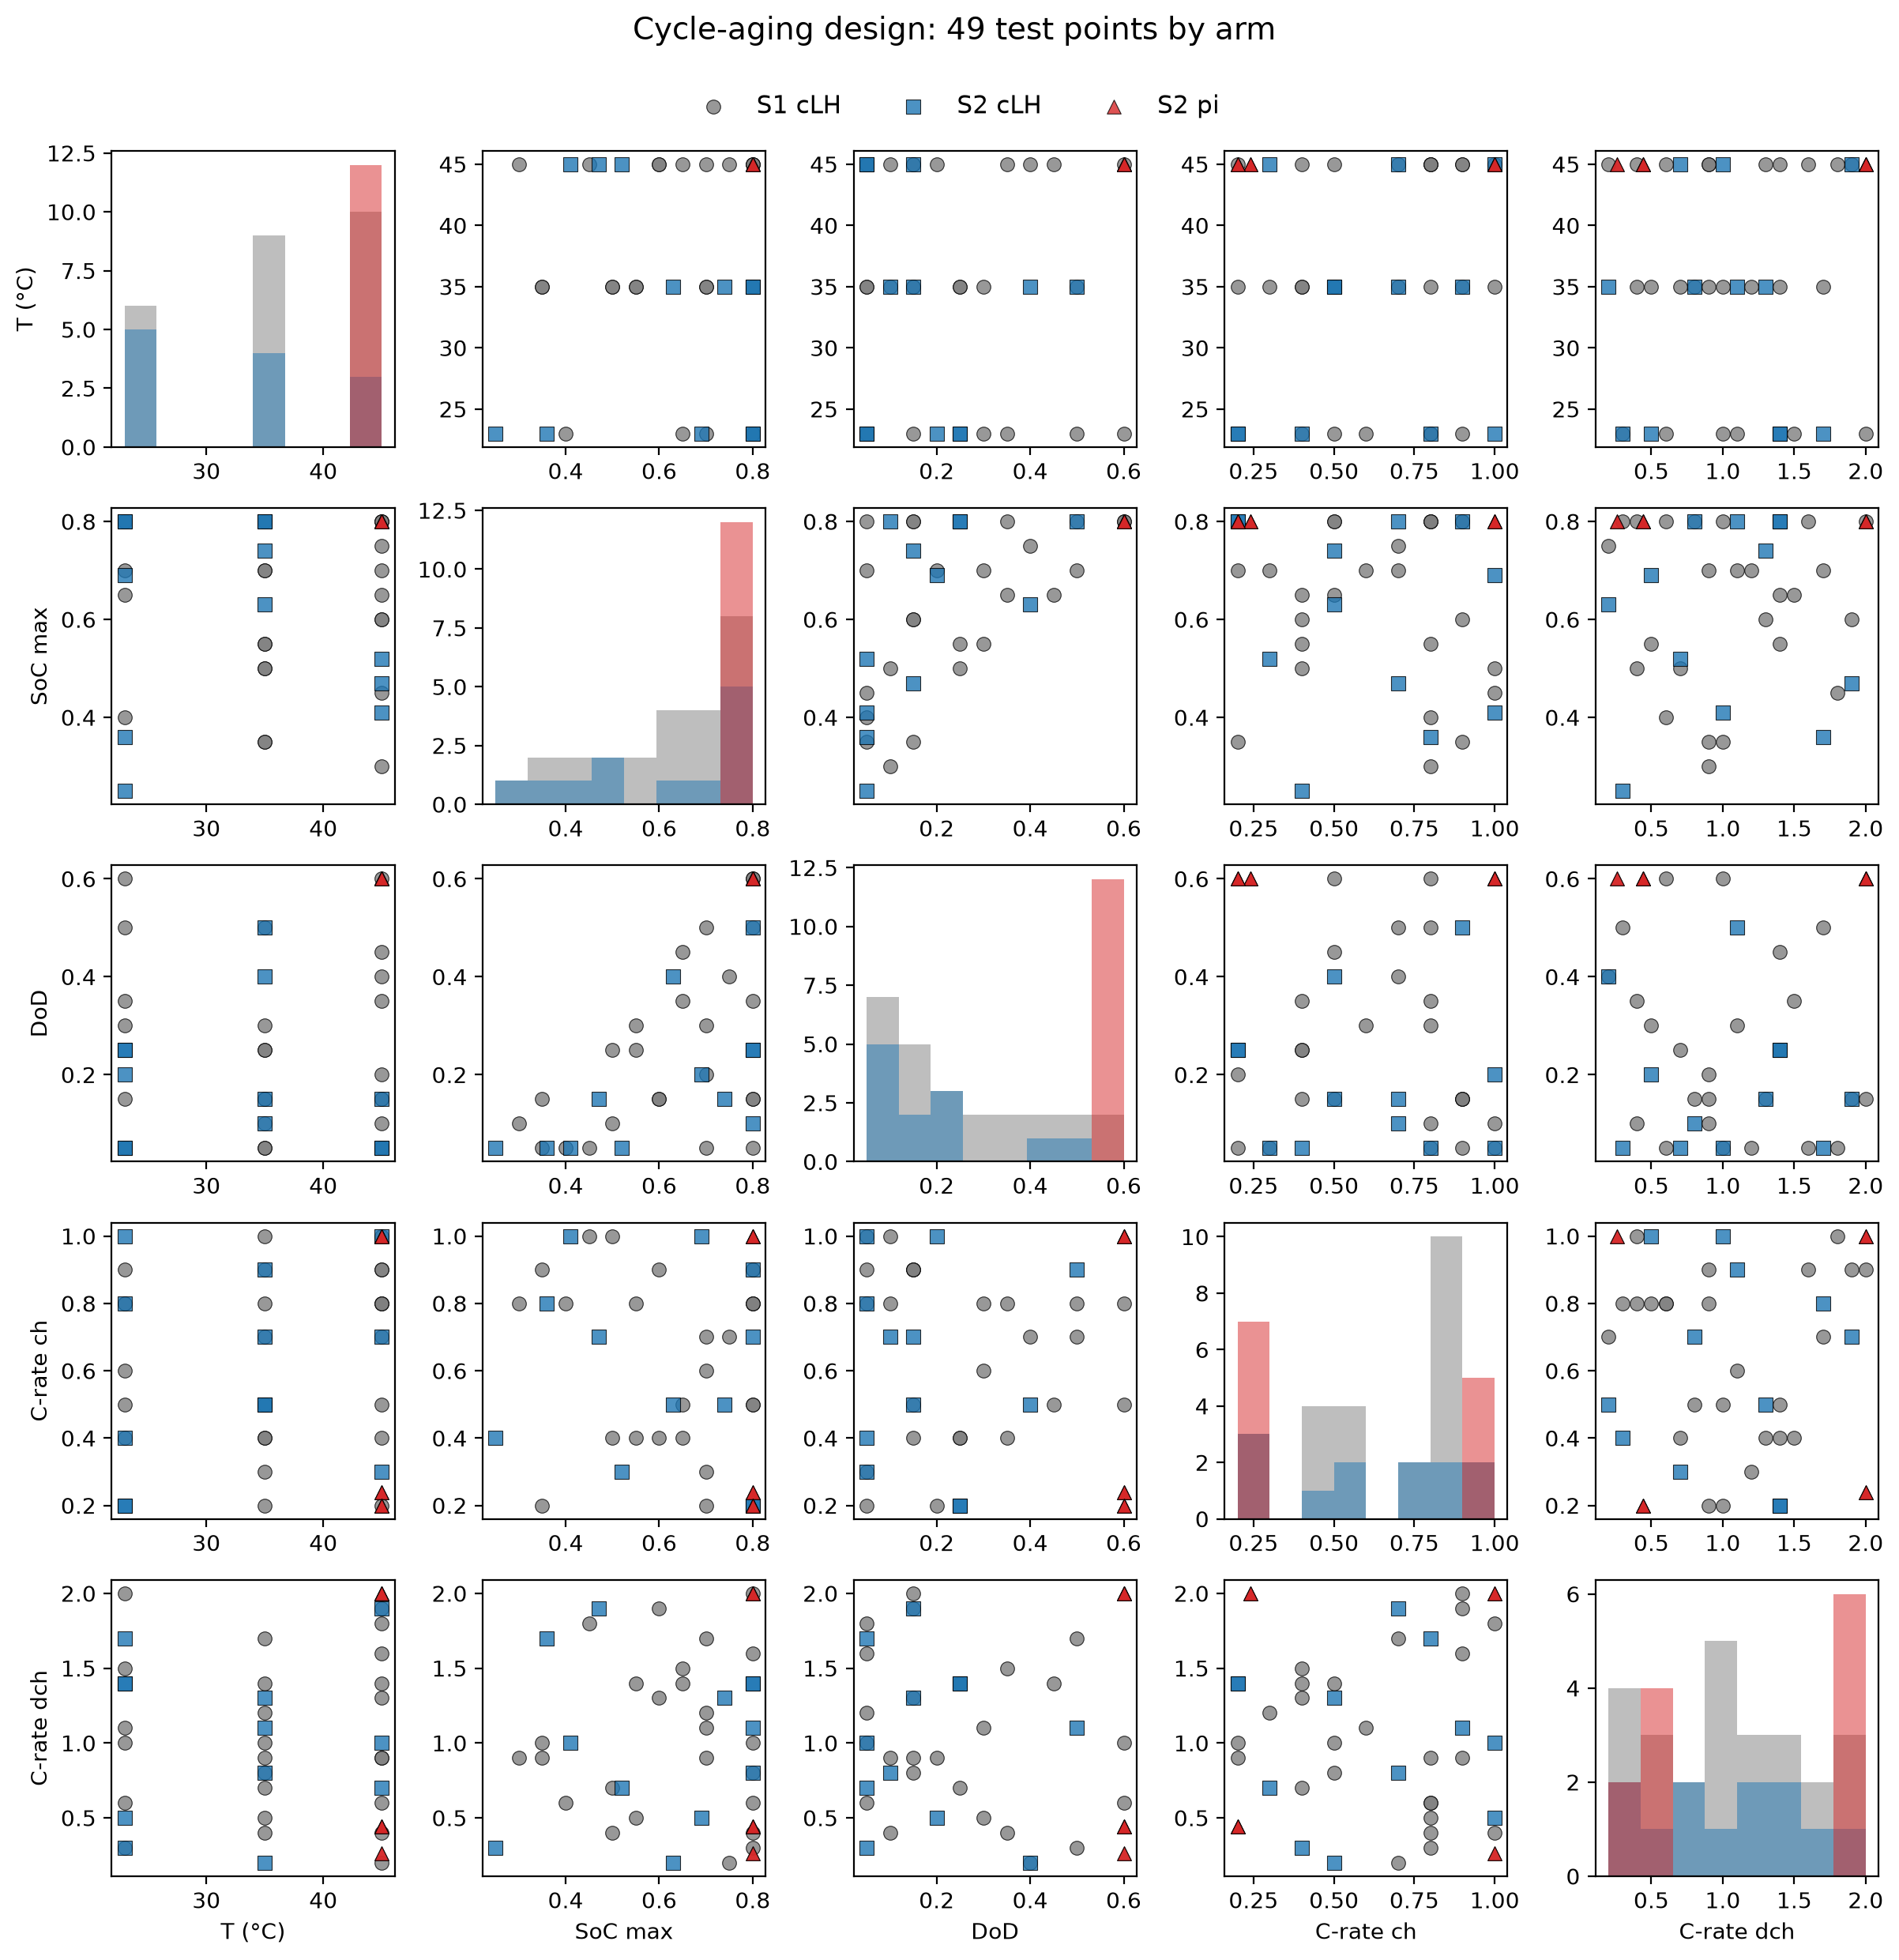
\includegraphics[width=0.82\textwidth]{fig0_cycle_design.png}
\caption{Cycle-aging design: the 49 test points by arm in every pair of the five stress factors (off-diagonal: scatter, $x$ = column factor, $y$ = row factor; diagonal: histogram of test points). Gray: S1 cLH pilot; blue: S2 cLH control; red: S2 pi-OED. All pi-OED points lie at $T=45\,^\circ$C, SoC$_{\max}=0.8$, DoD $=0.6$ and differ only in the two C-rates.}\label{fig:design}
\end{figure}

\subsection{Calendar aging}\label{sec:prelim-cal}
\Cref{fig:cal} shows the stage-1 calendar fade curves. Four features matter for the model \eqref{eq:cal}:
\begin{enumerate}
  \item \textbf{Temperature dominates.} Cells at 45\,$^\circ$C lose up to about 5\% of capacity in 260 days; at 10 and 23\,$^\circ$C the loss stays below about 2\%. This is the effect $\theta_0^{\mathrm{cal}}$ is meant to capture.
  \item \textbf{The SoC effect is non-monotonic at 45\,$^\circ$C.} SoC 80\% fades as fast as or faster than SoC 100\% for most of the test, the behavior that led the authors to restrict S2 to SoC $\le80\%$ \cite{stroebl2026}. The power law $(\mathrm{SoC}/\mathrm{SoC}_{\mathrm{ref}})^{\theta_1}$ cannot represent it.
  \item \textbf{10 and 23\,$^\circ$C look alike.} At SoC 100\%, both temperatures reach about 0.98 after roughly 250--300 days, whereas a single Arrhenius term predicts a clear gap. If this holds in the fit, $\theta_0^{\mathrm{cal}}$ is identified almost entirely by the 45\,$^\circ$C cells.
  \item \textbf{Replicates agree closely, and curves are concave} (steep early, flattening later), consistent with $t^{\theta_2}$, $\theta_2<1$.
\end{enumerate}

\begin{figure}[H]
\centering
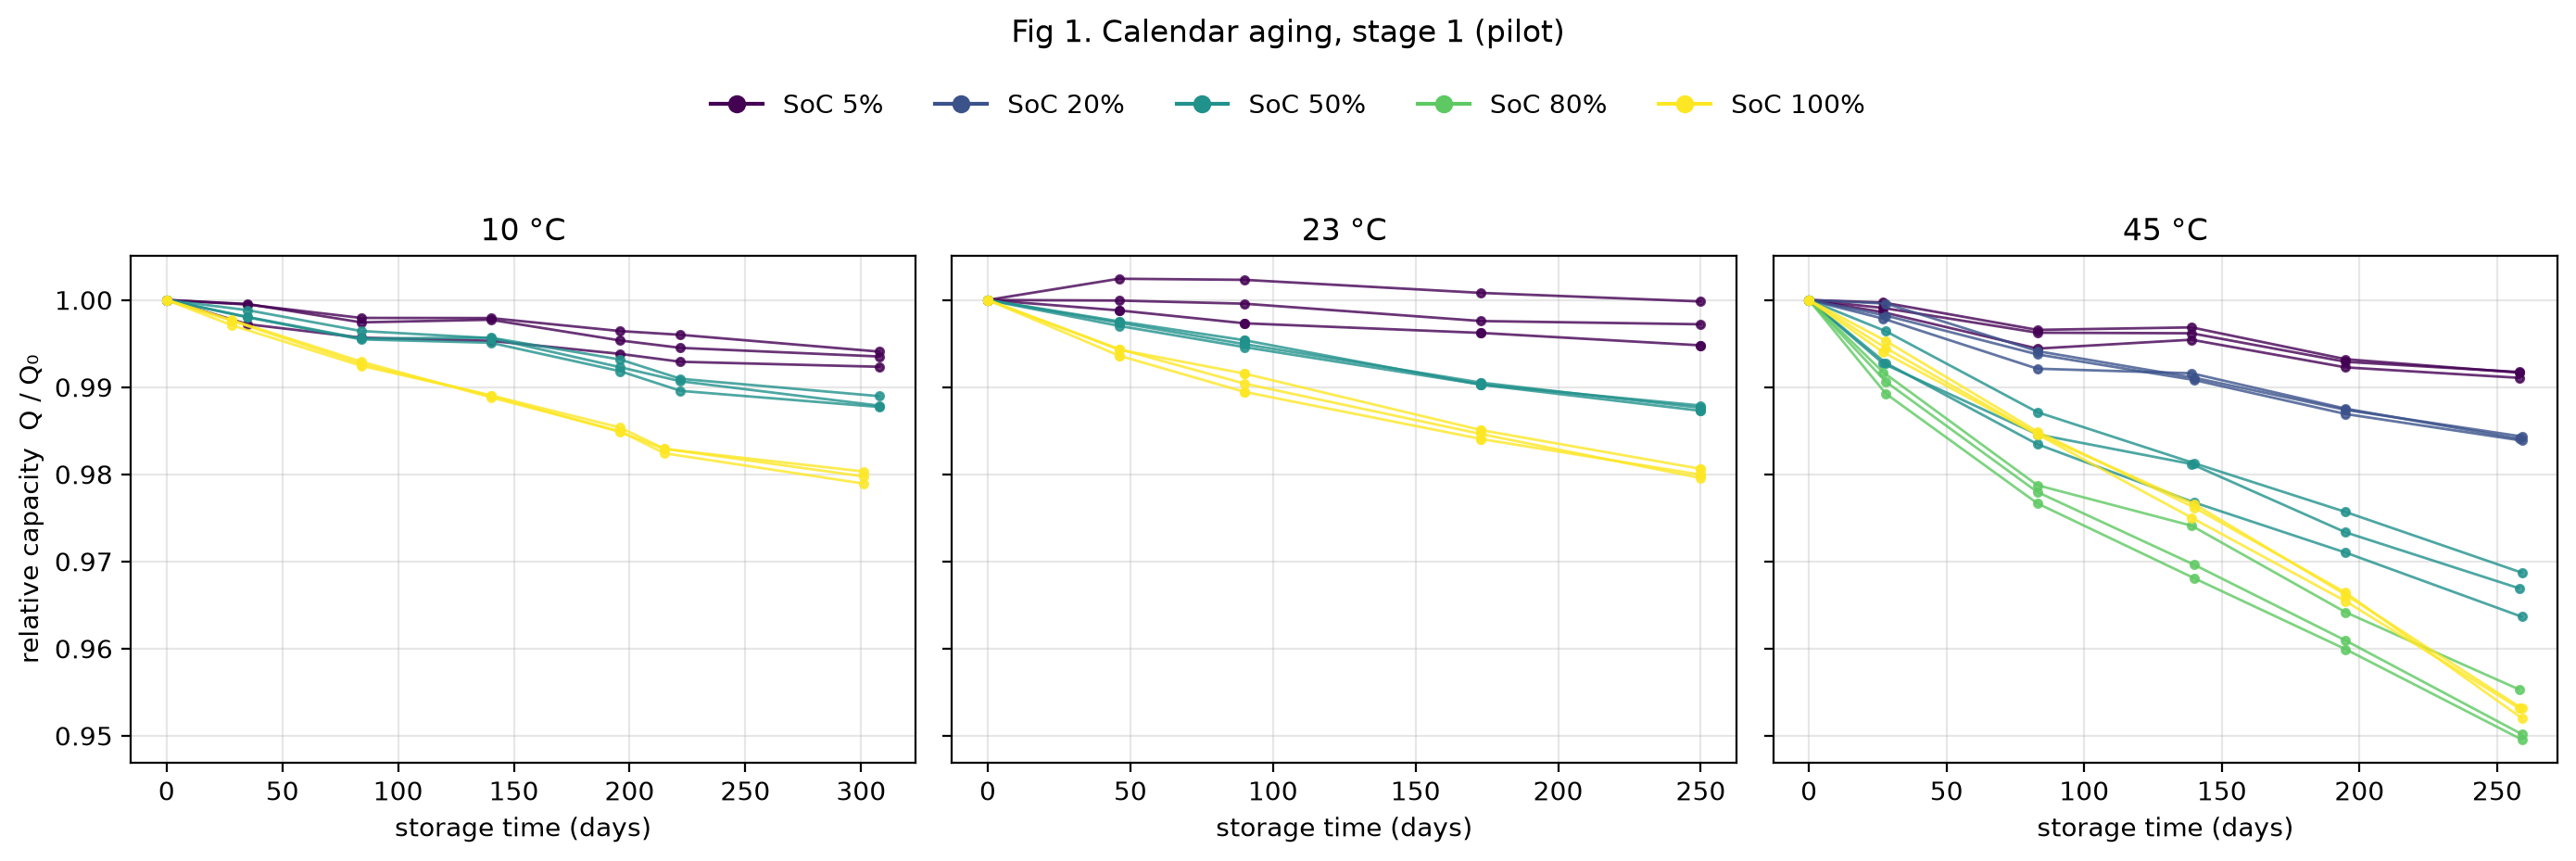
\includegraphics[width=\textwidth]{fig1_calendar_s1.png}
\caption{Calendar aging, stage 1: relative capacity vs.\ storage time, one panel per storage temperature, one line per cell, colored by storage SoC.}\label{fig:cal}
\end{figure}

\subsection{Cycle aging}\label{sec:prelim-cycle}
\Cref{fig:cyc} shows relative capacity against equivalent full cycles for the three cycle-aging arms. By their last RPT, cells reached between 336 and 4{,}888 EFC (median 1{,}628). The pi-OED cells fade much faster per cycle (about 0.88 at 1{,}500 EFC, where most S1 cells are still above 0.92); part of this is calendar aging at 45\,$^\circ$C accumulated during cycling, which the EFC axis does not separate. The pilot arm is heterogeneous and already contains the irregular trajectories the authors describe: one 23\,$^\circ$C cell falls to 0.93 within about 250 EFC, and one 45\,$^\circ$C cell bends sharply near 4{,}000 EFC to 0.78. One or two S2 control cells show a step drop near 2{,}300 EFC, which looks like a test interruption rather than aging and will be flagged before fitting.

\begin{figure}[H]
\centering
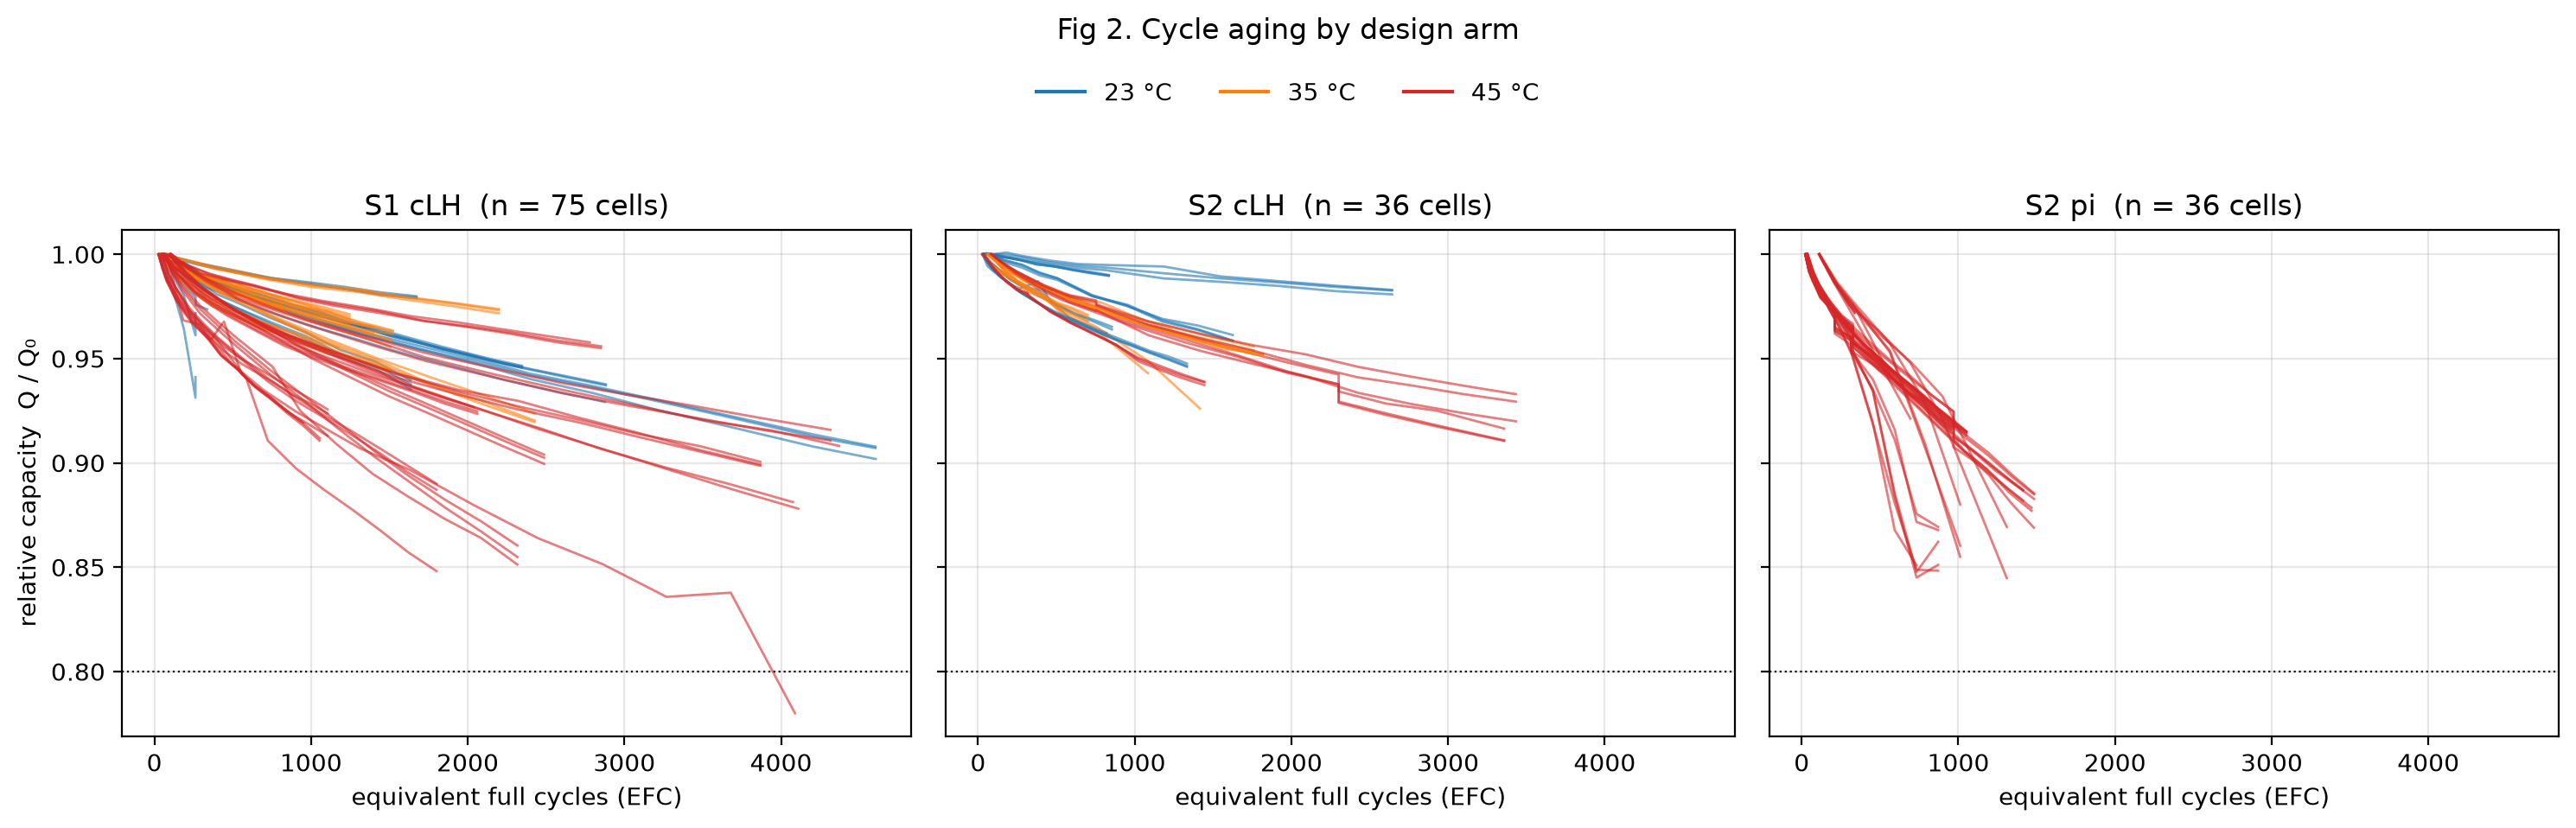
\includegraphics[width=\textwidth]{fig2_cycle_by_arm.png}
\caption{Cycle aging by design arm: relative capacity vs.\ equivalent full cycles (EFC), one line per cell, colored by ambient temperature. Dotted line: 80\% end-of-life threshold.}\label{fig:cyc}
\end{figure}

\Cref{fig:pi} separates the pi-OED arm by its four C-rate conditions, which all share the same temperature, SoC$_{\max}$, and DoD. The arm splits cleanly. Both low-charge-rate conditions ($C_{\mathrm{ch}}\approx0.2$) fade almost linearly with tight replicates. Both 1C-charge conditions show a \emph{knee}: with slow discharge (0.26C), the cells fade normally for about 350 EFC and then drop to about 0.85 by 700 EFC; with fast discharge (2.0C), the knee comes later (about 700--1{,}000 EFC) and is less consistent across cells. A plausible reading of the ordering is that slow discharge lengthens each cycle, so per EFC the cell spends more time at 45\,$^\circ$C and high SoC\dash an interaction between charge rate and time at temperature.

This bears directly on the published diagnosis. The authors found the targeted C-rate factors ``not statistically significant'' \cite{stroebl2026}. In the raw data the charge rate has a large effect at this corner, but a non-smooth one: a regime change that a power law in throughput with separable multiplicative factors cannot produce. A fit that averages knee and non-knee cells would let the C-rate parameters absorb the mismatch, which is consistent with the drift of $\theta_3$ from $-12.8$ to $-284.6$ and the tenfold growth of its SD. My working hypothesis is therefore that the cycle failure is primarily a model-adequacy (R1) failure at the design points OED chose, rather than an inherently insensitive factor. This is to be tested by fitting the published model with and without an interaction or knee term, and, for \RQ1, by asking whether stage-1 data alone\dash which include the single corner test point at 0.8C charge\dash already signal the problem.

\begin{figure}[H]
\centering
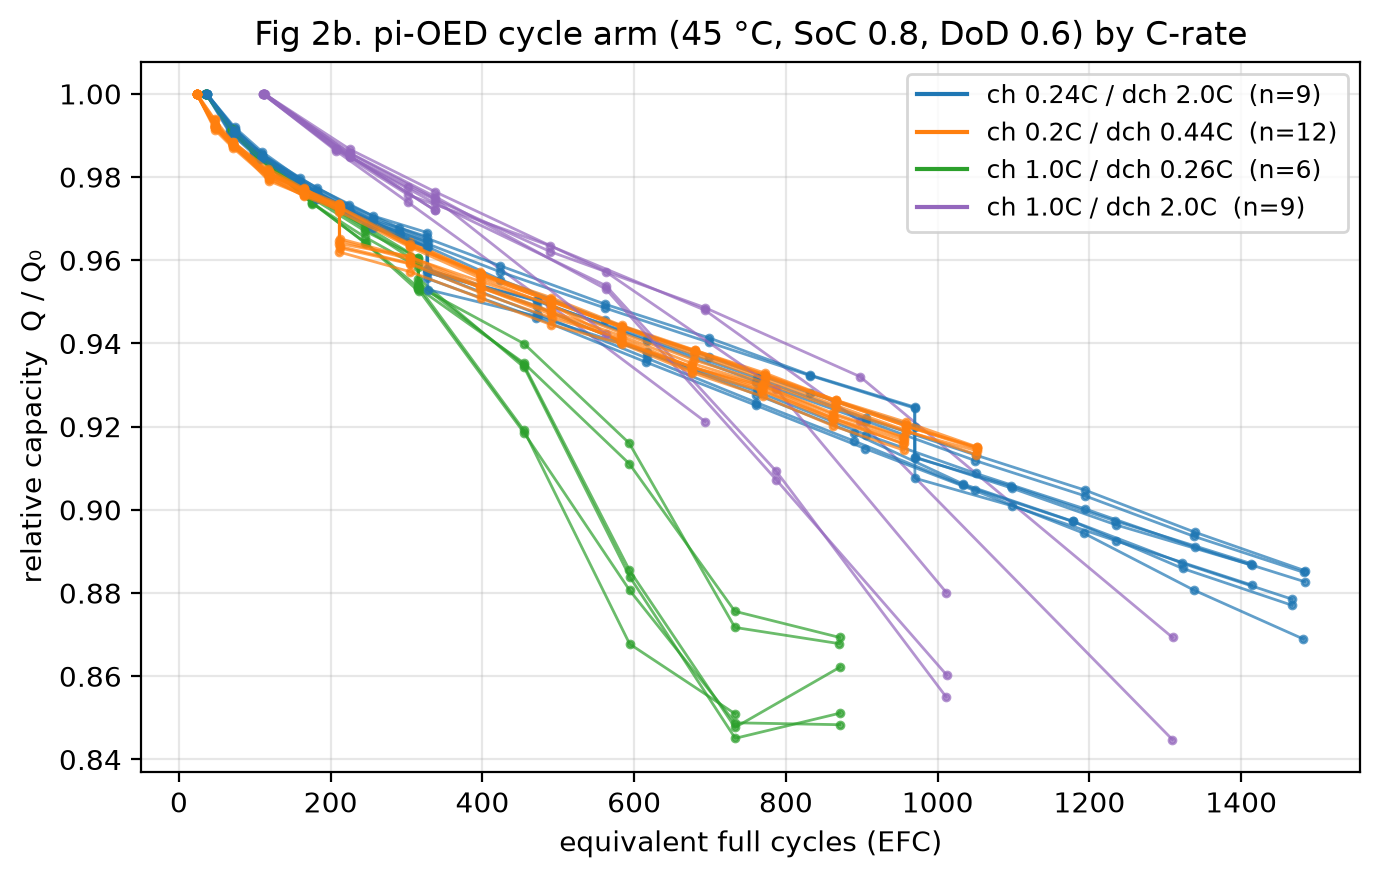
\includegraphics[width=0.72\textwidth]{fig2b_pi_by_crate.png}
\caption{The pi-OED cycle arm (45\,$^\circ$C, SoC$_{\max}$ 0.8, DoD 0.6) by C-rate condition; $n$ = number of cells. Both 1C-charge conditions develop a knee; the low-charge-rate conditions fade almost linearly.}\label{fig:pi}
\end{figure}

\subsection{Replicate noise}\label{sec:prelim-noise}
\Cref{fig:noise} plots, for every test point and RPT, the standard deviation of relative capacity across replicate cells against the mean capacity lost. This is a model-free first version of $D_3$: under the homoscedastic noise that the FIM \eqref{eq:fim} assumes, the cloud would be flat.
\begin{itemize}
  \item \textbf{Typical noise is small:} median replicate SD is 0.058\% of initial capacity for calendar and 0.106\% for cycle aging.
  \item \textbf{Calendar noise is flat} over its loss range (0--5\%): close to the FIM assumption.
  \item \textbf{Cycle noise grows with degradation,} from about 0.05\% below 2\% loss to about 0.3\% at 8--15\% loss, roughly proportional to the loss: heteroskedastic.
  \item \textbf{Cycle noise is heavy-tailed:} about 30 points sit at 1--7\%, 10--50 times the typical SD. They come from individual replicate cells diverging from their siblings (an early knee, or one cell aging far less), e.g.\ at one S1 test point one cell is at 0.966 after about 4{,}100 EFC while its two replicates are at about 0.88, and at one pi-OED condition replicates differ by about 0.09 at the same throughput.
\end{itemize}
Together with \cref{sec:prelim-cycle}, this gives a data-level counterpart of the R2 failure reported by the authors: calendar noise is light-tailed and roughly homoscedastic, where OED succeeded; cycle noise grows with degradation and has heavy tails driven by cell-to-cell differences in knee onset, where OED failed. It also argues for the random-effects term $b_{ij}$ in the model of \cref{sec:problem} and for heteroskedastic and heavy-tailed noise conditions in the \RQ2 simulation.

\begin{figure}[H]
\centering
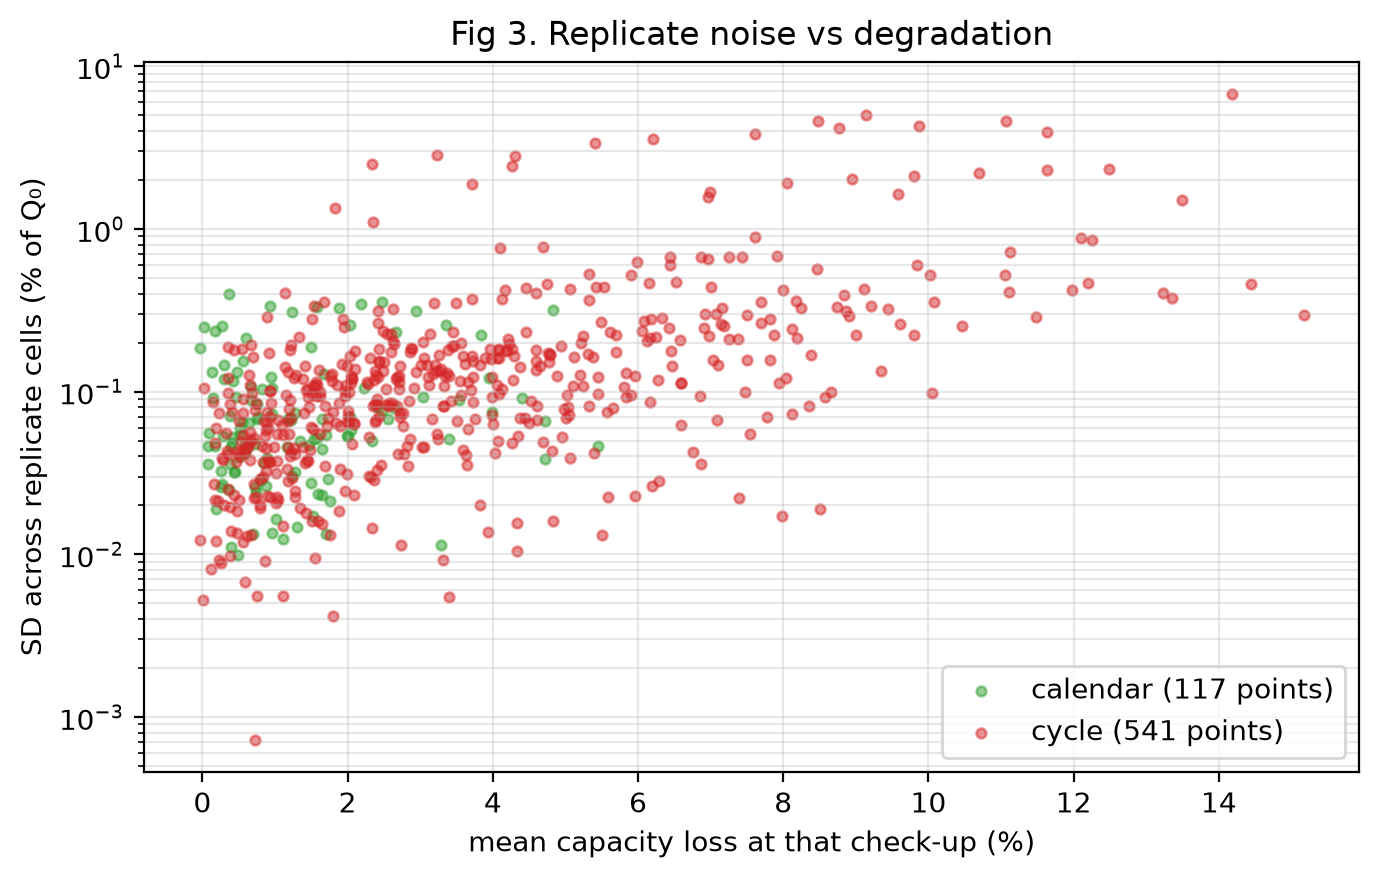
\includegraphics[width=0.72\textwidth]{fig3_replicate_noise.png}
\caption{Replicate noise vs.\ degradation: standard deviation of relative capacity across replicate cells at the same test point and RPT (log scale) against the mean capacity lost, for calendar (green) and cycle (red) test points with at least three replicates. RPTs are aligned by their order within each cell.}\label{fig:noise}
\end{figure}

\subsection{Implications for the planned analyses}
\begin{itemize}
  \item \textbf{\RQ1.} The calendar/cycle split already appears, model-free, in where the pi-OED points sit relative to the pilot data (interior and bracketed vs.\ an untested corner) and in the noise structure. Both motivate concrete, S1-computable statistics ($D_2$ support and interaction checks; $D_3$ variance-vs-level and tail weight). Because these observations used S2 data, the diagnostics will be finalized on S1 only and tested out of sample on Severson and Sandia.
  \item \textbf{\RQ2.} The simulation's noise levels and forms can now be set from data: SD of order 0.05--0.1\% of capacity, flat for calendar, growing with loss and heavy-tailed for cycle aging, with 3--6 replicates per condition.
  \item \textbf{\RQ3.} The cycle pi-OED arm is an extreme concentrated design; a compromise design that keeps some cells away from the corner, or a maximin design over models with and without a charge-rate interaction, is a concrete counterfactual to evaluate.
  \item \textbf{Next.} Reproduce the published S1 fits (Tables D.2--D.3); then compute $D_1$ (FIM spectra) for both sub-studies.
\end{itemize}

% =====================================================================
\section{Expected Results, Deliverables, and Limitations}\label{sec:expected}
\begin{itemize}
  \item \textbf{Expected:} $D_1$--$D_3$ separate the calendar and cycle arms on S1 data alone; bootstrap intervals under-cover at Stroebl-scale sample sizes while profile-likelihood intervals hold; compromise designs avert the cycle failure at a modest efficiency cost in the calendar case. A null result on any item is itself informative and reportable.
  \item \textbf{Deliverables:} the three analyses above; a one-page practitioner checklist answering the ``checklist-style thresholds'' request in \cite{stroebl2026}; open code and data pipeline.
  \item \textbf{Limitations:} counterfactual designs cannot be run on real cells within the thesis; conclusions about model discrepancy depend on the hyper-model chosen; one primary chemistry (NMC 21700) for the main validation; and the exploratory analysis of \cref{sec:prelim} has seen the Stroebl S2 outcomes, so the Stroebl validation of \RQ1 is retrospective rather than blind (mitigated by fixing diagnostics on S1 only and testing out of sample on Severson and Sandia).
\end{itemize}

\section{Conclusion}
OED for battery aging has passed from promise to a documented split result. This thesis proposes to make the method \emph{certifiable}: to say from pilot data whether it will help, to say whether its uncertainty statements can be trusted, and to design so that it cannot badly fail. Each question is answerable on public data with tools that sit squarely in statistical inference and constrained optimization; the first look at the Stroebl data (\cref{sec:prelim}) suggests that the cycle-aging failure has visible, quantifiable signatures in the design and the noise.

% =======================================
\newpage
\addcontentsline{toc}{section}{References}
\begin{thebibliography}{99}\small

\bibitem{stroebl2026} F.~Stroebl, F.~Schaeufl, O.~Bohlen, H.~Palm, ``Model-based optimal experimental design for lithium-ion battery aging: Insights from a comprehensive multi-stage study with real-world data,'' \emph{Journal of Energy Storage} \textbf{142}:119552 (2026). \url{https://doi.org/10.1016/j.est.2025.119552}

\bibitem{stroebl2024} F.~Stroebl, R.~Petersohn, B.~Schricker, F.~Schaeufl, O.~Bohlen, H.~Palm, ``A multi-stage lithium-ion battery aging dataset using various experimental design methodologies,'' \emph{Scientific Data} \textbf{11} (2024). \url{https://doi.org/10.1038/s41597-024-03859-z} Data: \url{https://doi.org/10.6084/m9.figshare.25975315}

\bibitem{palm2022} N.~Palm, F.~Stroebl, H.~Palm, ``Parameter individual optimal experimental design and calibration of parametric models,'' \emph{IEEE Access} \textbf{10}:112515--112528 (2022). \url{https://doi.org/10.1109/ACCESS.2022.3216364} Code: \url{https://github.com/nicolaipalm/oed}

\bibitem{mathieu2017} R.~Mathieu, I.~Baghdadi, O.~Briat, P.~Gyan, J.-M.~Vinassa, ``D-optimal design of experiments applied to lithium battery for ageing model calibration,'' \emph{Energy} \textbf{141}:2108--2119 (2017).

\bibitem{forman2012} J.~C.~Forman, S.~J.~Moura, J.~L.~Stein, H.~K.~Fathy, ``Optimal experimental design for modeling battery degradation,'' \emph{ASME Dynamic Systems and Control Conference}, DSCC2012-MOVIC2012-8751 (2012).

\bibitem{benmarzouk2016} M.~Ben-Marzouk, A.~Chaumond, E.~Redondo-Iglesias, M.~Montaru, S.~P\'elissier, ``Experimental protocols and first results of calendar and/or cycling aging study of lithium-ion batteries\dash the MOBICUS project,'' \emph{World Electric Vehicle Journal} \textbf{8}, EVS29 (2016).

\bibitem{movahedi2023} H.~Movahedi, S.~Pannala, J.~B.~Siegel, A.~G.~Stefanopoulou, ``Physics-informed optimal experiment design of calendar aging tests and sensitivity analysis for SEI parameters estimation in lithium-ion batteries,'' \emph{IFAC-PapersOnLine} \textbf{56}(3):433--438 (2023). \url{https://www.sciencedirect.com/science/article/pii/S2405896323023959}

\bibitem{park2018} S.~Park, D.~Kato, Z.~Gima, R.~Klein, S.~Moura, ``Optimal experimental design for parameterization of an electrochemical lithium-ion battery model,'' \emph{J.\ Electrochem.\ Soc.} (2018). \url{https://ecal.studentorg.berkeley.edu/pubs/ParamID-ConvexOED.pdf}

\bibitem{pozzi2019} A.~Pozzi, G.~Ciaramella, S.~Volkwein, D.~M.~Raimondo, ``Optimal design of experiments for a lithium-ion cell: parameters identification of a single particle model with electrolyte dynamics,'' arXiv:1811.08656 (2019). \url{https://arxiv.org/abs/1811.08656}

\bibitem{ozkan2025} M.~F.~Ozkan, S.~Filgueira da Silva, F.~El Idrissi, P.~Ramesh, M.~Canova, ``Optimal design of experiment for electrochemical parameter identification of Li-ion battery via deep reinforcement learning,'' arXiv:2506.19146 (2025). \url{https://arxiv.org/abs/2506.19146}

\bibitem{mikesell2025} I.~Mikesell, S.~Filgueira da Silva, M.~F.~Ozkan, F.~El Idrissi, P.~Ramesh, M.~Canova, ``Real-time optimal design of experiment for parameter identification of Li-ion cell electrochemical model,'' arXiv:2504.15578 (2025). \url{https://arxiv.org/abs/2504.15578}

\bibitem{roman2022} L.~A.~Rom\'an-Ram\'irez, J.~Marco, ``Design of experiments applied to lithium-ion batteries: A literature review,'' \emph{Applied Energy} (2022). \url{https://www.sciencedirect.com/science/article/pii/S0306261922006596}

\bibitem{white2016} A.~White, M.~Tolman, H.~D.~Thames, H.~R.~Withers, K.~A.~Mason, M.~K.~Transtrum, ``The limitations of model-based experimental design and parameter estimation in sloppy systems,'' arXiv:1602.05135 (2016); \emph{PLoS Comput.\ Biol.} \url{https://arxiv.org/abs/1602.05135}

\bibitem{qibaker2025} J.~Qi, R.~E.~Baker, ``Optimal experimental design for parameter estimation in the presence of observation noise,'' arXiv:2504.19233 (2025). \url{https://arxiv.org/abs/2504.19233}

\bibitem{limyum2011} H.~Lim, B.-J.~Yum, ``Optimal design of accelerated degradation tests based on Wiener process models,'' \emph{Journal of Applied Statistics} \textbf{38}(2):309--325 (2011). \url{https://doi.org/10.1080/02664760903406488}

\bibitem{amini2018} M.~Amini, S.~Shemehsavar, Z.~Pan, ``Optimal design for step-stress accelerated test with random discrete stress elevating times based on gamma degradation process,'' arXiv:1404.3806 (2014/2018). \url{https://arxiv.org/abs/1404.3806}

\bibitem{shen2018} D.~Shen, T.~Liu, L.~Zhang, J.~Wang, Y.~Liu, ``A novel accelerated degradation test design considering stress optimization,'' \emph{Cluster Computing} \textbf{22}:S8793--S8802 (2019). \url{https://doi.org/10.1007/s10586-018-1970-0}

\bibitem{shi2017} Y.~Shi, B.~Xu, Y.~Tan, B.~Zhang, ``A convex cycle-based degradation model for battery energy storage planning and operation,'' arXiv:1703.07968 (2017); \emph{American Control Conference} (2018). \url{https://arxiv.org/abs/1703.07968}

\bibitem{xu2018} B.~Xu, J.~Zhao, T.~Zheng, E.~Litvinov, D.~S.~Kirschen, ``Factoring the cycle aging cost of batteries participating in electricity markets,'' \emph{IEEE Trans.\ Power Systems} \textbf{33}(2):2248--2259 (2018). \url{https://arxiv.org/abs/1707.04567}

\bibitem{chaloner1995} K.~Chaloner, I.~Verdinelli, ``Bayesian experimental design: A review,'' \emph{Statistical Science} \textbf{10}(3):273--304 (1995).

\bibitem{severson2019} K.~A.~Severson et al., ``Data-driven prediction of battery cycle life before capacity degradation,'' \emph{Nature Energy} \textbf{4}:383--391 (2019). \url{https://doi.org/10.1038/s41560-019-0356-8} Data: \url{https://data.matr.io/1/}

\bibitem{preger2020} Y.~Preger et al., ``Degradation of commercial lithium-ion cells as a function of chemistry and cycling conditions,'' \emph{J.\ Electrochem.\ Soc.} \textbf{167}:120532 (2020). \url{https://doi.org/10.1149/1945-7111/abae37} Data: \url{https://www.batteryarchive.org}

\bibitem{wang2011} J.~Wang et al., ``Cycle-life model for graphite-LiFePO$_4$ cells,'' \emph{J.\ Power Sources} \textbf{196}(8):3942--3948 (2011).

\bibitem{vetter2005} J.~Vetter et al., ``Ageing mechanisms in lithium-ion batteries,'' \emph{J.\ Power Sources} \textbf{147}:269--281 (2005).

\bibitem{ramadan2025} M.~S.~Ramadan, M.~Barrera, M.~Anitescu, S.~Herbert, ``Simultaneous improvement of control and estimation for battery management systems,'' arXiv:2507.21300 (2025). \url{https://arxiv.org/abs/2507.21300}

\bibitem{na2024} S.~Na, M.~Anitescu, M.~Kolar, ``A fast temporal decomposition procedure for long-horizon nonlinear dynamic programming,'' \emph{Mathematics of Operations Research} \textbf{49}(2):1012--1044 (2024). \url{https://doi.org/10.1287/moor.2023.1378}

\bibitem{na2023} S.~Na, M.~Anitescu, M.~Kolar, ``Inequality constrained stochastic nonlinear optimization via active-set sequential quadratic programming,'' \emph{Mathematical Programming} (2023).

\bibitem{dou2019} X.~Dou, M.~Anitescu, ``Distributionally robust optimization with correlated data from vector autoregressive processes,'' \emph{Operations Research Letters} \textbf{47}(4):294--299 (2019). \url{https://doi.org/10.1016/j.orl.2019.04.005}

\bibitem{petra2017} N.~Petra, C.~G.~Petra, Z.~Zhang, E.~M.~Constantinescu, M.~Anitescu, ``A Bayesian approach for parameter estimation with uncertainty for dynamic power systems,'' \emph{IEEE Trans.\ Power Systems} (2017).

\end{thebibliography}
\end{document}
